% Déclaration du type de document (report, book, paper, etc...)
\documentclass[a4paper]{report} 
 
% Package pour avoir Latex en français
\usepackage[utf8]{inputenc}
\usepackage[frenchb]{babel}
 
% Quelques packages utiles
\usepackage{listings} % Pour afficher des listings de programmes
\usepackage{graphicx} % Pour afficher des figures
\usepackage{amsthm}   % Pour créer des théorèmes et des définitions
\usepackage{amsmath}
\usepackage{microtype} % Optical margins FTW
\usepackage{url}
\usepackage{booktabs} % Allows the use of \toprule, \midrule and \bottomrule in tables for horizontal lines
\usepackage{siunitx}
\usepackage{floatrow}
\usepackage{caption}
\usepackage{subcaption}

% Début du document
\begin{document}

\begin{titlepage}

\newcommand{\HRule}{\rule{\linewidth}{0.5mm}} % Defines a new command for the horizontal lines, change thickness here

\center % Center everything on the page 
%----------------------------------------------------------------------------------------
%	HEADING 
%----------------------------------------------------------------------------------------
\textsc{\LARGE École Polytechnique Fédérale de~Lausanne}\\[1.5cm] 
\textsc{\Large Méthodes de Production}\\[0.5cm] % Major heading such as course name

%----------------------------------------------------------------------------------------
%	TITLE 
%----------------------------------------------------------------------------------------
\HRule \\[0.4cm]
{ \huge \bfseries Molded Interconnect Devices}\\[0.4cm] % Title of your document
\HRule \\[1.5cm]
 
%----------------------------------------------------------------------------------------
% LOGO EPFL
%----------------------------------------------------------------------------------------
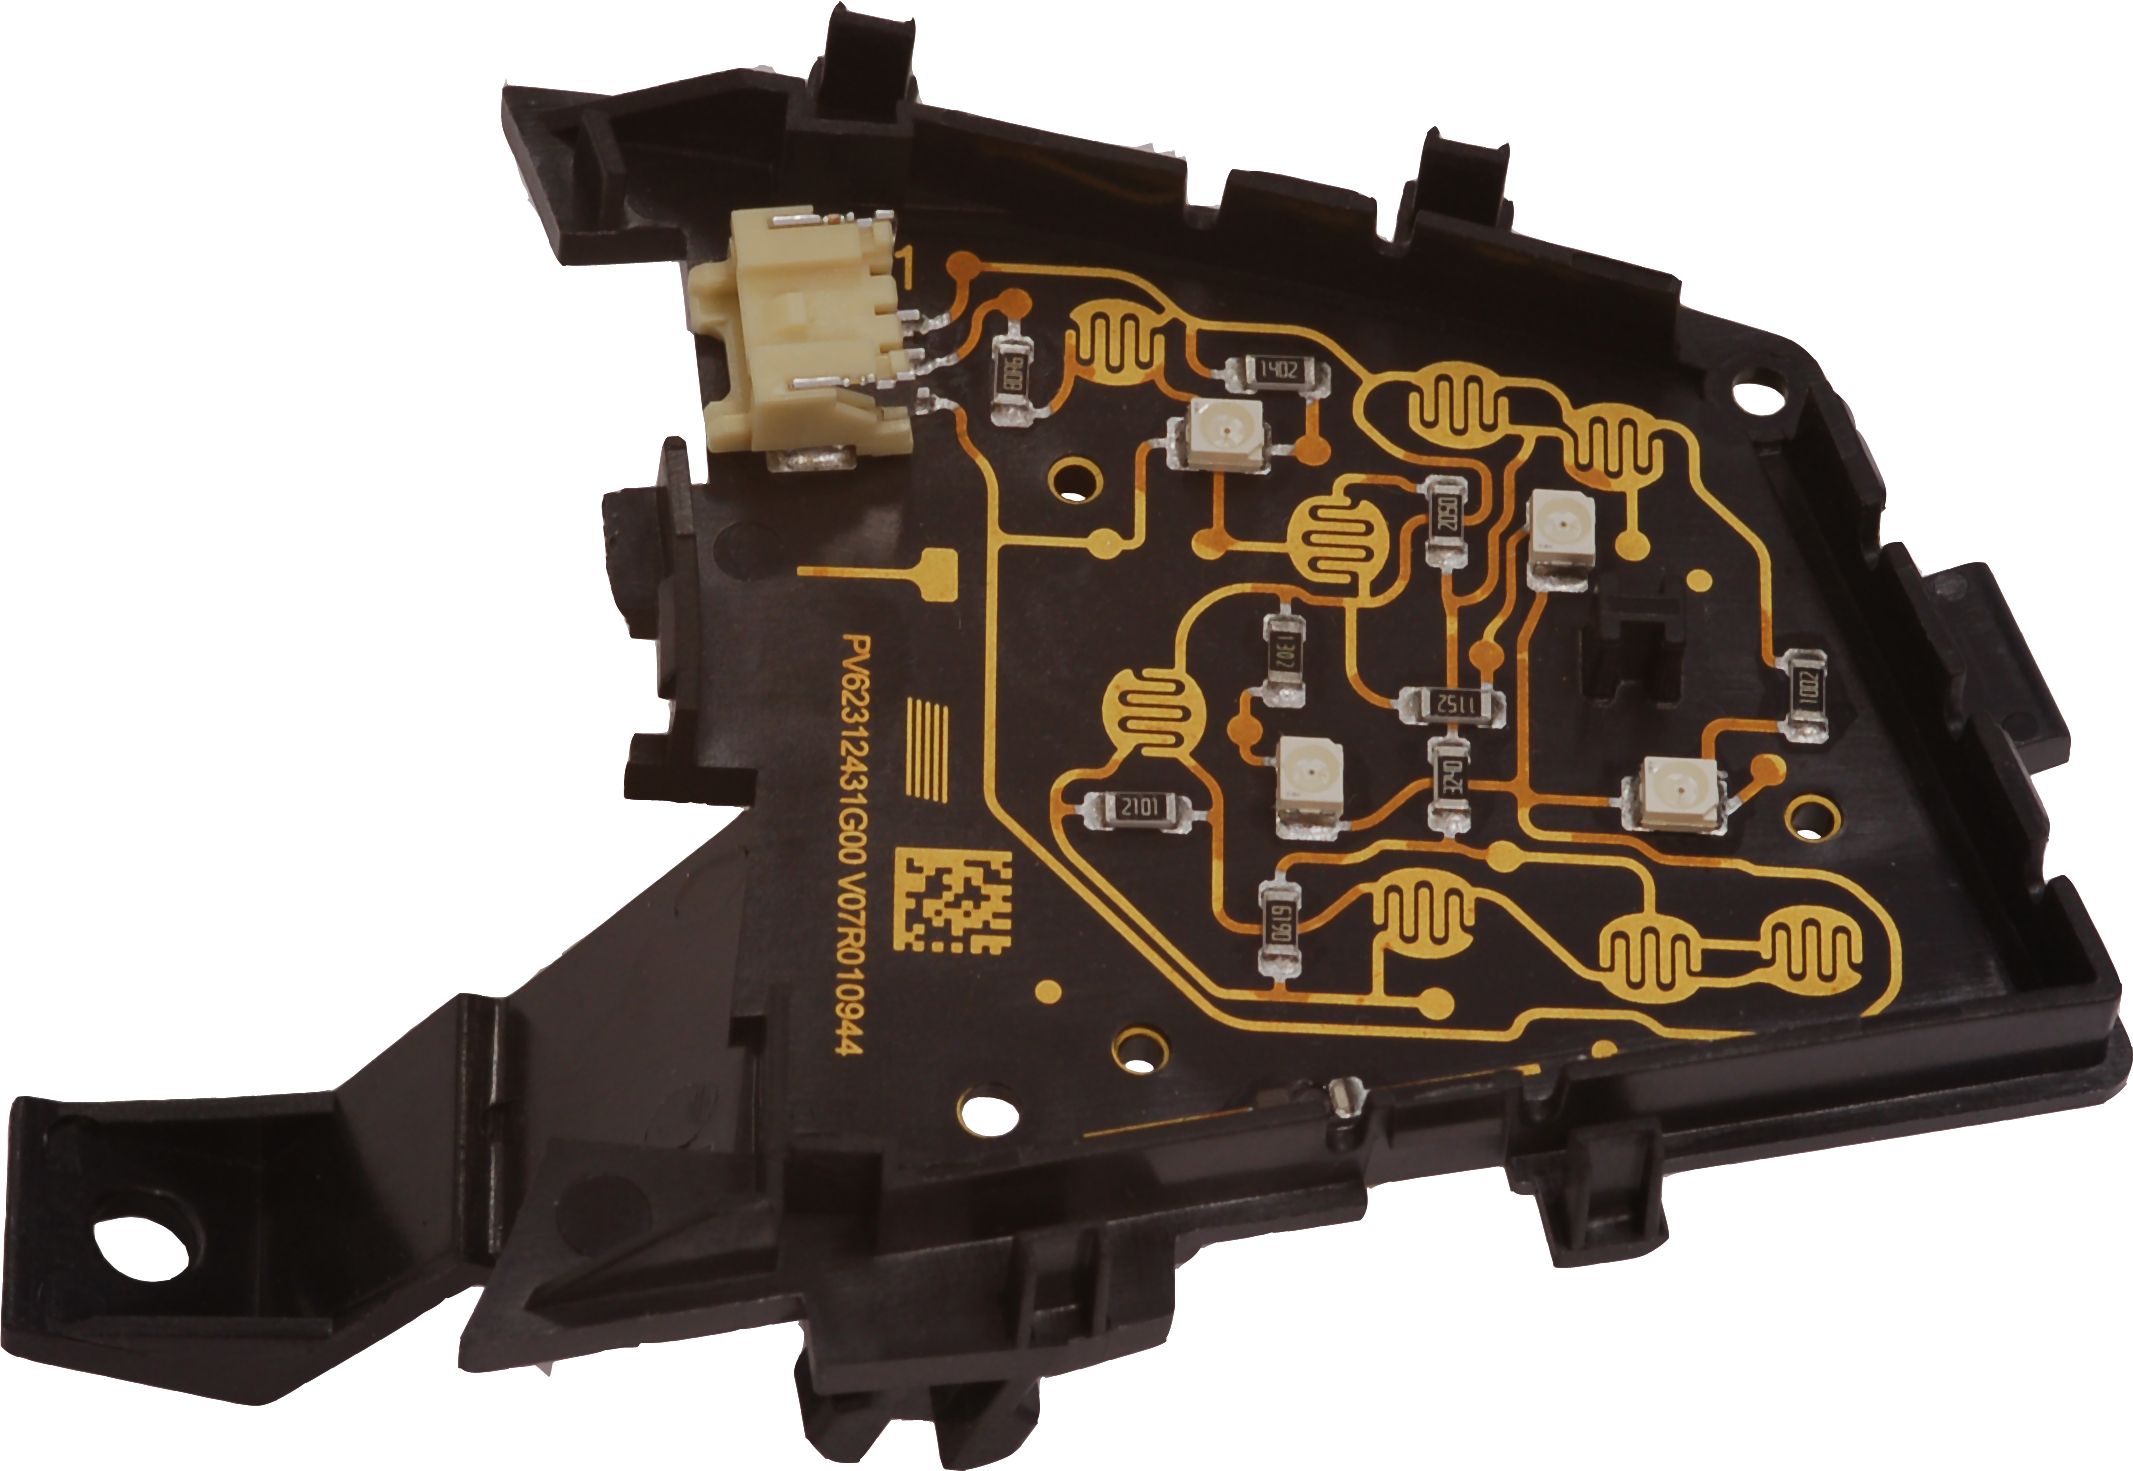
\includegraphics[width=0.8\textwidth]{../images/mid_example}\\[2cm]

%----------------------------------------------------------------------------------------
%	AUTHORS 
%----------------------------------------------------------------------------------------

\vfill % Fill the rest of the page with whitespace
\begin{minipage}{0.55\textwidth}
\begin{flushleft} \large
\emph{Étudiants:}\\
Antoine \textsc{Albertelli}\\ 
Quentin \textsc{Herzig}
\end{flushleft}
\end{minipage}
~
\begin{minipage}{0.4\textwidth}
\begin{flushleft} \large
\emph{Enseignants:} \\
Pr. Jacques \textsc{Jacot} \\
Pr. Peter \textsc{Ryser}\\
Dr. Jean-Daniel \textsc{Lüthi}
\end{flushleft}
\end{minipage}\\[2cm]


{\large 13 décembre 2013}
\end{titlepage}

% Empty page after title page.
\begin{titlepage}
    ~
\end{titlepage}



\tableofcontents

\clearpage
\section{Introduction}
Un \gls{mid}  est un circuit électronique
dont le support est un substrat thermoplastique moulé par injection, par
opposition au \textsc{PCB} conventionnels dont le substrat est un composite
plat.

Les \gls{mid} permettent de regrouper dans une seule pièce des fonctions
mécaniques et éléctroniques. En effet, contrairement au \textsc{pcb} conventionnels, les
\gls{mid} peuvent être conçus en trois dimensions, ce qui réduit
considérablement le nombre de composants et de connecteurs, diminuant ainsi le
temps d'assemblage, et donc le coût du système. 

Les \gls{mid}s ne sont toutefois pas une solution de remplacement des
\textsc{pcb}s car ils ne permettent pas une grande densité de pistes, tandis que
les \textsc{pcb}s à plus de deux couches sont désormais peu coûteux et
permettent des circuits à forte densité.


\begin{figure}
        \centering
        \begin{subfigure}[b]{0.4\textwidth}
                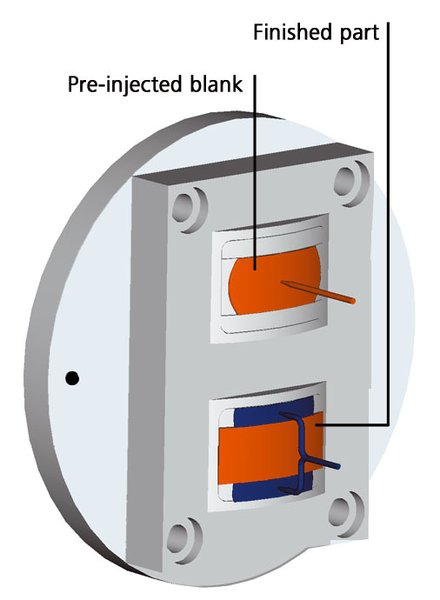
\includegraphics[width=\textwidth]{two-shots-a}
                \caption{Remplissage simultané des moules}
                \label{fig:gull}
        \end{subfigure}%
        ~ 
        \begin{subfigure}[b]{0.4\textwidth}
                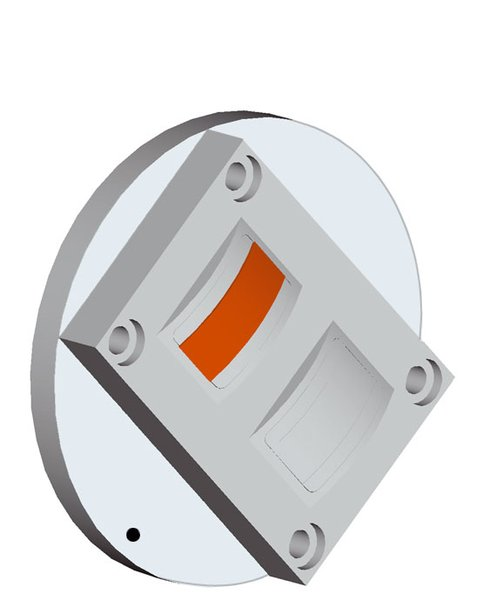
\includegraphics[width=\textwidth]{two-shots-b}
                \caption{Rotation des moules}
                \label{fig:lol}
        \end{subfigure}%
        \caption{Procedé two-shot}\label{fig:animals}

        \floatfoot{Source: \url{http://www.sumitomo-shi-demag.eu/processes/multi-component-technology/rotary-plate.html}}
\end{figure}

\appendix
\listoffigures

\nocite{*} % tells bibtex to include everything
\bibliographystyle{abbrv-fr}
\bibliography{biblio}
\end{document}
